\documentclass[11pt, a4paper, twoside]{article}   	% use "amsart" instead of "article" for AMSLaTeX format

\usepackage{geometry}                		% See geometry.pdf to learn the layout options. There are lots.
\usepackage{pdfpages}
\usepackage{caption}
\usepackage{minted}
\usepackage[german]{babel}			% this end the next are needed for german umlaute
\usepackage[utf8]{inputenc}
\usepackage{color}
\usepackage{graphicx}
\usepackage{titlesec}
\usepackage{fancyhdr}
\usepackage{lastpage}
\usepackage{hyperref}
\usepackage[autostyle=false, style=english]{csquotes}
\usepackage{mathtools}
\usepackage{tabularx}
% http://www.artofproblemsolving.com/wiki/index.php/LaTeX:Symbols#Operators
% =============================================
% Layout & Colors
% =============================================
\geometry{
   a4paper,
   total={210mm,297mm},
   left=20mm,
   right=20mm,
   top=20mm,
   bottom=30mm
 }	

\definecolor{myred}{rgb}{0.8,0,0}
\definecolor{mygreen}{rgb}{0,0.6,0}
\definecolor{mygray}{rgb}{0.5,0.5,0.5}
\definecolor{mymauve}{rgb}{0.58,0,0.82}

\setcounter{secnumdepth}{4}


% the default java directory structure and the main packages
\newcommand{\srcDir}{../src/}
% =============================================
% Code Settings
% =============================================
\newenvironment{code}{\captionsetup{type=listing}}{}
\newmintedfile[mSourceFile]{matlab}{
	linenos=true, 
	frame=single, 
	breaklines=true, 
	tabsize=2,
	numbersep=5pt,
	xleftmargin=10pt,
	baselinestretch=1,
	fontsize=\footnotesize
}
\newmintinline[mInlineSource]{matlab}{}
\newminted[mSource]{matlab}{
	breaklines=true, 
	tabsize=2,
	autogobble=true,
	breakautoindent=false
}
% =============================================
% Page Style, Footers & Headers, Title
% =============================================
\title{Übung 1}
\author{Thomas Herzog}

\lhead{Übung 1}
\chead{}
\rhead{
\includegraphics[scale=0.10]{FHO_Logo_Students.jpg}}

\lfoot{S1610454013}
\cfoot{}
\rfoot{ \thepage / \pageref{LastPage} }
\renewcommand{\footrulewidth}{0.4pt}
% =============================================
% D O C U M E N T     C O N T E N T
% =============================================
% =============================================
% 2016.10.13: 1 
% 2016.10.14: 2
% =============================================

\pagestyle{fancy}
\begin{document}
\setlength{\headheight}{15mm}
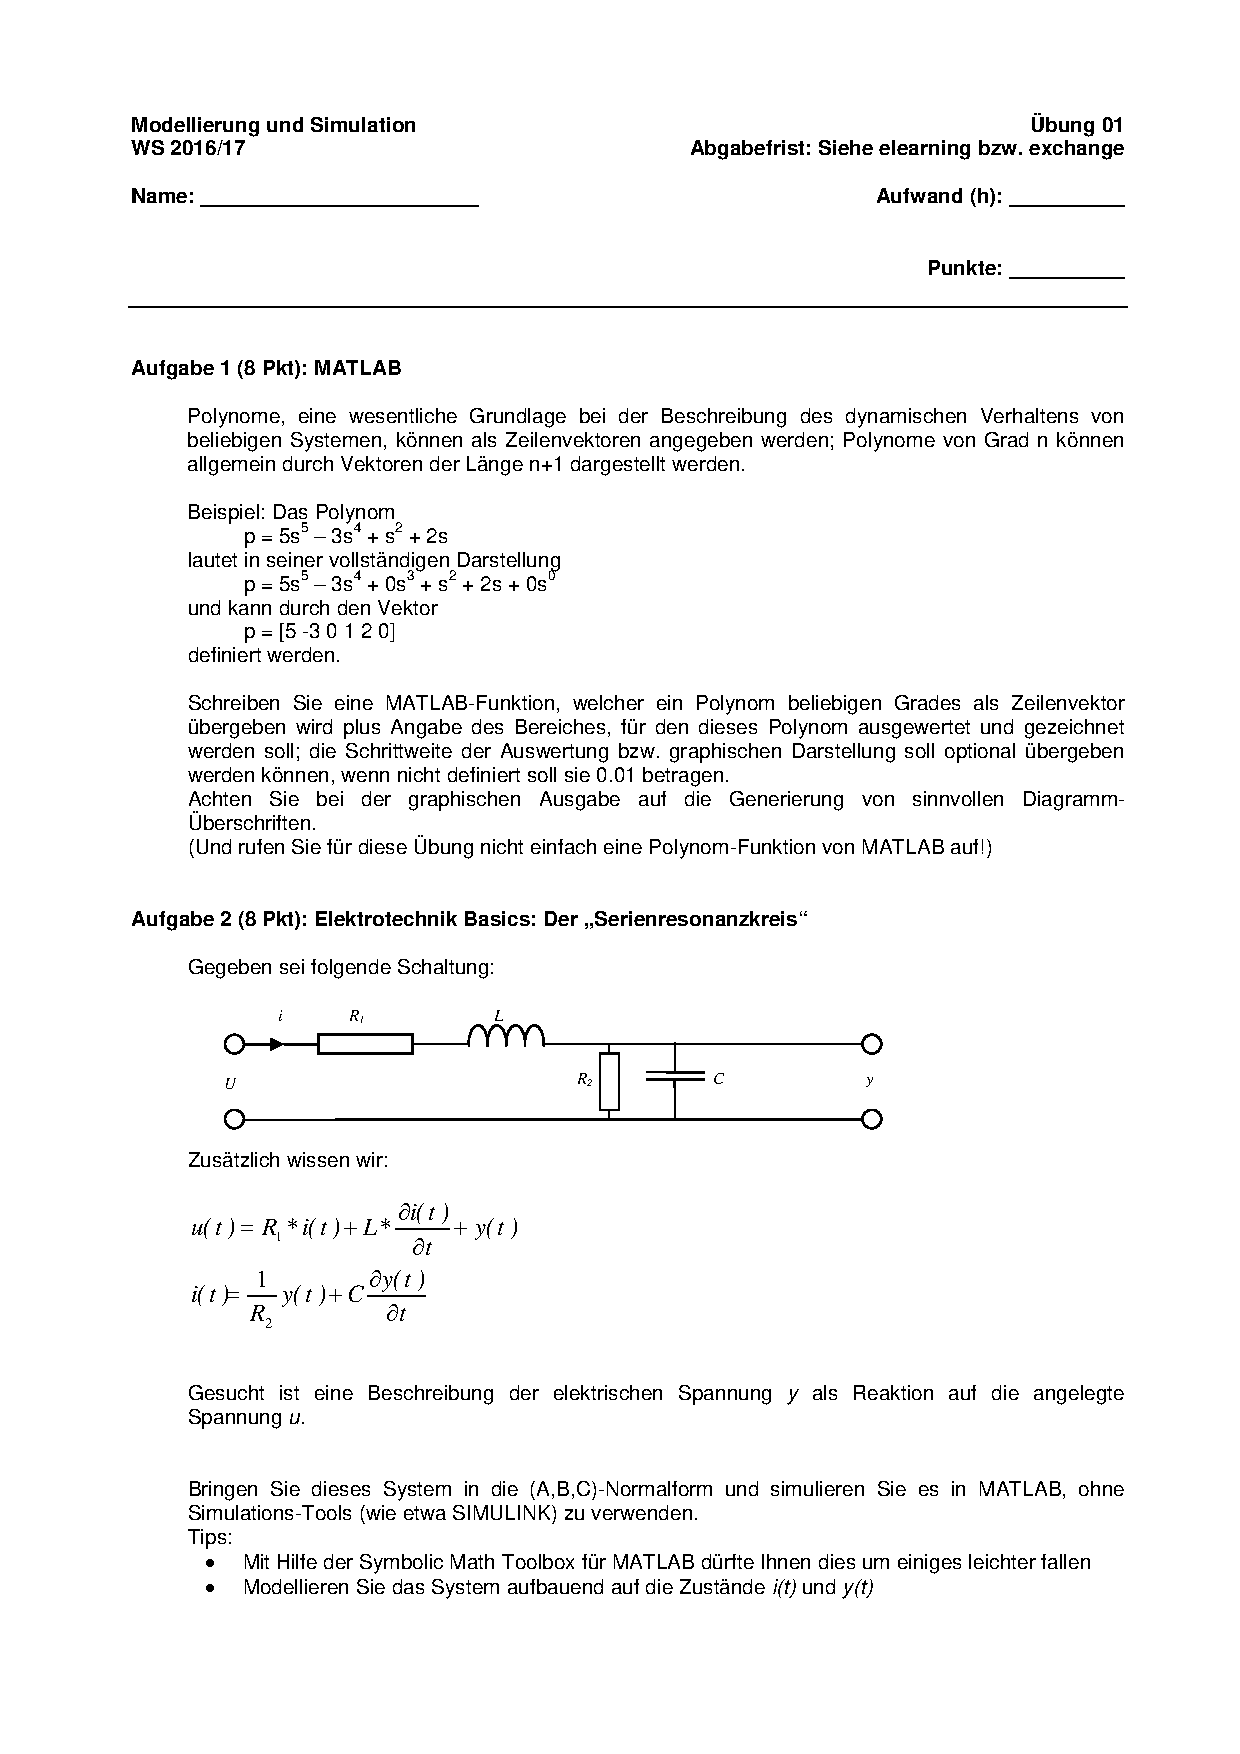
\includepdf[pages={1,2}]{Uebungszettel01.pdf}

% Section gramar and basics 
\section {Matlab}
\label{sec:matlab}
Dieser Abschnitt beschäftigt sich mit der Aufgabenstellung 1 der ersten Übung. Folgende Quelltexte zeigen die \emph{Matlab} Funktionen, die für diesen Teil der Übung implementiert wurden.
\newline
\newline
In die Funktion \emph{printPolynom} wurden Prüfungen der übergebenen Argumente implementiert wie
\begin{itemize}
	\item\emph{Gültigkeit der Argumentanzahl}
	\item\emph{Gültigkeit des Vektors}
	\item\emph{Gültigkeit der übergebenen Grenzen und Schrittweite}
\end{itemize}
\ \newline
Wenn die Schrittweite nicht gegeben ist, dann wird der Standardwert $0.01$ verwendet.
\begin{code}
	\caption{Funktion zum Plotten eines Polynoms des Grades n}
	\mSourceFile{\srcDir/printPolynom.m}
\end{code}
\begin{code}
	\caption{Funktion zum Umwandeln eines Polynoms des Grades n in eine Zeichenklette}
	\mSourceFile{\srcDir/poly2Str.m}
	\label{fig:print-poly}
\end{code}
\ \newline
Die Funktion aus dem Quelltext \ref{fig:print-poly} zeigt die Funktion, die implementiert wurde, um die Polynomfunktion repräsentiert durch einen Zeilenvektor in seine Repräsentation mit einer Zeichenkette zu konvertieren. Dies war erforderlich, da die Funktion \emph{poly2Sym} nicht zur Verfügung stand.
\newpage

\section{Der Serienresonanzkreis}
Dieser Abschnitt beschäftigt sich mit der Aufgabenstellung 2 der ersten Übung. 
\newline
\newline
Umformen der Gleichung nach $\check{i}(t)$.
\newline
\newline
\begin{tabularx}{\textwidth}{p{120pt} @{$=$ \hspace{10pt}} X X}
	$u(t)$  & $R_{1} * i(t) + L * \dfrac{\delta i(t)}{\delta t} + y(t)$ \\
	$u(t)$  & $R_{1} * i(t) + L * \check{i}(t) + y(t)$ & $\dfrac{\delta i(t)}{\delta t} = \check{i}(t)$ \\
	$u(t) - R_{1} * i(t) - y(t)$  & $L * \check{i}(t)$ & $- R_{1} * i(t) - y(t))$ \\
	$\dfrac{1}{L} * u(t) - \dfrac{R_{1}}{L} * i(t) - \dfrac{1}{L} * y(t)$  & $\check{i}(t)$ & $/ L$  \\
\end{tabularx}
\ \newline
\newline
$\check{i}(t) = \dfrac{1}{L} * u(t) - \dfrac{R_{1}}{L} * i(t) - \dfrac{1}{L} * y(t)$
\newline
\newline
\newline
\newline
Umformen der Gleichung nach $\check{y}(t)$.
\newline
\newline
\begin{tabularx}{\textwidth}{p{120pt} @{$=$ \hspace{10pt}} X X}
	$i(t)$  & $\dfrac{1}{R_{2}} * y(t) + C * \dfrac{\delta y(t)}{\delta t}$ \\
	$i(t)$  & $\dfrac{1}{R_{2}} * y(t) + C * \check{y}(t)$ & $\dfrac{\delta y(t)}{\delta t} = \check{y}(t)$\\
	$i(t) - \dfrac{1}{R_{2}} * y(t)$  & $C * \check{y}(t)$ & $- \dfrac{1}{R_{2}} * y(t)$ \\
	$\dfrac{1}{C} * i(t) - \dfrac{1}{C * R_{2}} * y(t)$  & $\check{y}(t)$ & $/ C$ \\
\end{tabularx}
\ \newline
\newline
$\check{y}(t) = \dfrac{1}{C} * i(t) - \dfrac{1}{C * R_{2}} * y(t)$
\newline
\newline
\newline
\newline
Substitution von $i(t), y(t)$
\newline
\newline
$x_{1}(t) = i(t)$
\newline
\newline
$x_{2}(t) = y(t)$
\newline
\newline
$\check{x_{1}}(t) = - \dfrac{R_{1}}{L} * x_{1}(t) - \dfrac{1}{L} * x_{2}(t) + \dfrac{1}{L} * u(t)$
\newline
$\check{x_{2}}(t) = \dfrac{1}{C} * x_{1}(t) - \dfrac{1}{C * R_{2}} * x_{2}(t) + 0 * u(t)$
\newline
\newline
\newline
\newline
$A, B, C$ Matrizen aufstellen:
\newline
\newline
$
A = \begin{bmatrix}
	\frac{R_{1}}{L} & -\frac{1}{L} \\[0.3em]
    \frac{1}{C}     & -\frac{1}{C*R_{2}} \\[0.3em]
\end{bmatrix}
,
B =  \begin{bmatrix}
	\frac{1}{L} \\[0.3em]
	0
\end{bmatrix}
,
C =  \begin{bmatrix}
	0 & 1 \\[0.3em]
\end{bmatrix}
$
\newpage
\parindent0pt In $A, B, C$ Normalform bringen:
\newline
\newline
$
\check{X}(t) = 
\begin{bmatrix}
	\frac{R_{1}}{L} & -\frac{1}{L} \\[0.3em]
    \frac{1}{C}     & -\frac{1}{C*R_{2}} \\[0.3em]
\end{bmatrix}
 * X(t) + 
\begin{bmatrix}
	\frac{1}{L} \\[0.3em]
	0
\end{bmatrix}
 * U(t)
$
\newline
\newline
\newline
$
Y(t) = 
\begin{bmatrix}
	0 & 1 \\[0.3em]
\end{bmatrix}
 *X(t)
$
\newpage
\section{Theorie der Kontinuierlichen Modellierung}
Dieser Abschnitt beschäftigt sich mit der Aufgabenstellung 3 der ersten Übung.
\subsection{3a Beschreibung der A,B,C Methode}
Dieser Abschnitt beschäftigt sich mit der Beschreibung der $A, B, C$ Methode.
\newline
\newline
Die $A, B, C$ Normalform beschreibt \emph{Linear Differential Systems}. Die Matrizen $A, B, C$ enthalten die Faktoren mit denen Eingangs-, Ausgangs- und Zustandsvariablen beeinflusst werden. 
\newline
\newline
\textbf{$A$-Matrix} ist die Matrix, welche die Faktoren der gegenseitigen Beeinflussung enthält. Diese Matrix beschreibt die gegenseitige Beeinflussung der inneren Zustände. Die $A$-Matrix hat so viele Spalten wie es innere Zustandsvariablen gibt, die in der $X(0)$-Matrix durch die Anzahl der Zeilen gegeben ist.
\newline
\newline
$
A = \begin{bmatrix}
	\frac{R_{1}}{L} & -\frac{1}{L} \\[0.3em]
    \frac{1}{C}     & -\frac{1}{C*R_{2}} \\[0.3em]
\end{bmatrix}
X(0) =
\begin{bmatrix}
	1  \\[0.3em]
    10 \\[0.3em]
\end{bmatrix} 
$
\newline
\newline
\newline
\textbf{$B$-Matrix} ist die Matrix, welche die Faktoren der Beeinflussung der Eingangsvariablen enthält. Diese Matrix beschreibt die Beeinflussung der Eingangsvariablen, die in der $U(t)$-Matrix durch die Anzahl der Zeilen gegeben ist.
\newline
\newline
$
B = \begin{bmatrix}
	\frac{R_{1}}{L} \\[0.3em]
	0
\end{bmatrix}
U(t) =
\begin{bmatrix}
	1  \\[0.3em]
\end{bmatrix} 
$
\newline
\newline
\newline
\textbf{$C$-Matrix} ist die Matrix, die aufgestellt wird, je nachdem welchen Output man erhalten will. Die $c$-Matrix wird in der Ausgangsgleichung $y(t) = C*x(t)$ verwendet. Die Anzahl der Spalten ergibt sich aus der Anzahl der Zeilen der Ausgangsmatrix, die angibt wie viele Ausgangsvariablen es gibt. Die Werte $0$ und $1$ in der $C$-Matrix werden verwendet um die einzelnen Ausgangsvariabeln bei der Betrachtung miteinzubeziehen oder auszuschließen.
\newline
\newline
$
C_{i(t)} = \begin{bmatrix}
	1 & 0\\[0.3em]
\end{bmatrix}
*
X(t) =
\begin{bmatrix}
	i(t)  \\[0.3em]
	y(t)
\end{bmatrix}$
\hspace{1mm}
$|$
\hspace{1mm}
$
C_{y(t)} = \begin{bmatrix}
	0 & 1\\[0.3em]
\end{bmatrix}
*
X(t) =
\begin{bmatrix}
	i(t)  \\[0.3em]
	y(t)
\end{bmatrix} 
$
\hspace{1mm}
$|$
\hspace{1mm}
$
C_{y(t)} = \begin{bmatrix}
	1 & 1\\[0.3em]
\end{bmatrix}
*
X(t) =
\begin{bmatrix}
	i(t)  \\[0.3em]
	y(t)
\end{bmatrix} 
$
\newline
\newline
\newline
Hat man sein System auf die $A, B, C$ Normalform gebracht, kann man die einzelnen Werte mit dem Integral ausrechnen, das sich durch die Umformung der $A, B, C$ Normalform ergibt, wenn der Zustand $X(0)$ bekannt ist.
\newline
\newline
Diese mathematische Beschreibung zeigt, die Zusammenhänge und Beeinflussung der Variablen innerhalb des Systems. Mit der $A, B, C$ Normalform, kann die Veränderung eines Zustands im System zum Zeitpunkt $t$ berechnet werden.
\newline
\newline
Die Simulationssoftware verwendet die Berechnungsmethoden intern um auf die graphische Darstellung zu kommen, also kann es keine Simulationssoftware geben, die nicht auf Grundlage dieser Berechnungsmethoden arbeitet.
\newpage
\subsection{3b Zusammenhang der Formeln der A, B, C Methode}
Dieser Abschnitt beschäftigt sich mit der Beschreibung des Zusammenhangs der Formeln der $A, B, C$ Methode.
\newline
\newline


\end{document}